\documentclass{standalone}
\usepackage{pgfplots}
\usepackage{tikz}
\usetikzlibrary{
        angles,
        quotes,
    }

\newcommand{\gridCirc}[2]{
\addplot[thick,data cs=polar,domain=0:360,samples=360,smooth,#2] (x,#1);
}

\newcommand{\constCirc}[4]{

\addplot[thick,data cs=polar,domain=0:360,samples=#1+1,smooth,mark=*, only marks,#4] (x+#3,#2);
}

\definecolor{blue}{rgb}{0,0.4470,0.7410}
\definecolor{red}{rgb}{0.8500,0.3250,0.0980}


\begin{document}





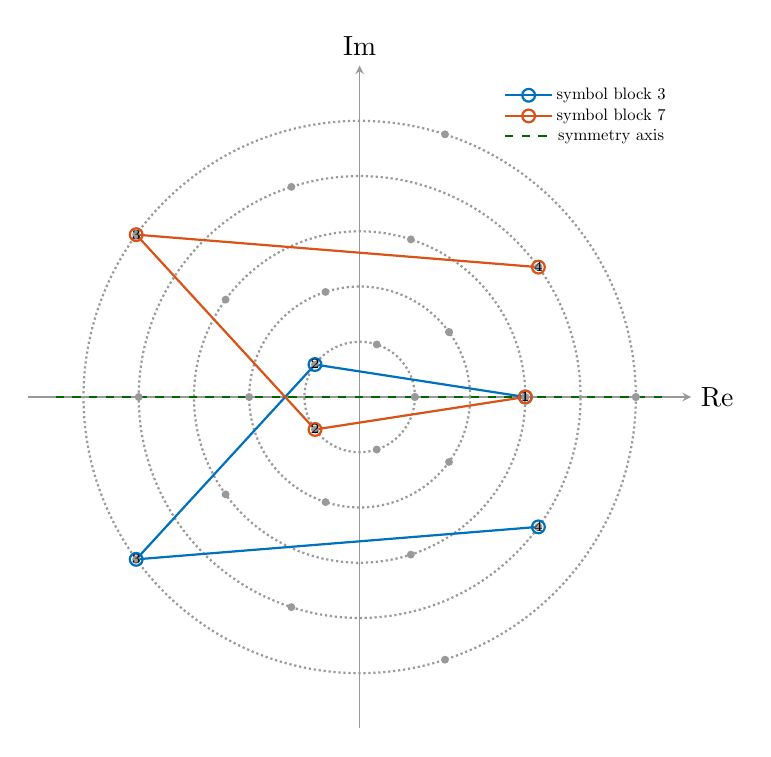
\begin{tikzpicture}[>= stealth]
\begin{axis}[
  width = 10cm,
  height = 10cm,
  xlabel={$t$},
  axis x line=middle,  % Show only the x-axis
  axis y line=middle,    % Hide the y-axis
  xmin=-6, xmax=6,
  ymin=-6, ymax=6,  % Set ymax to 2
  xtick=\empty,
  ytick=\empty,
  xlabel = Re,
  ylabel = Im,
  xlabel style={
    right,black
  },
  ylabel style={
    above,black
  },
  legend style={draw=none,nodes={scale=0.6, transform shape},
  every axis/.append style={%
      black!40
    }   },  
]


\gridCirc{1}{black!40, densely dotted, forget plot,}
\constCirc{5}{1}{0}{black!40, mark size=1pt, forget plot}
\gridCirc{2}{black!40, densely dotted, forget plot,}
\constCirc{5}{2}{36}{black!40, mark size=1pt, forget plot}
\gridCirc{3}{black!40, densely dotted, forget plot,}
\constCirc{5}{3}{0}{black!40, mark size=1pt, forget plot}
\gridCirc{4}{black!40, densely dotted, forget plot,}
\constCirc{5}{4}{36}{black!40, mark size=1pt, forget plot}
\gridCirc{5}{black!40, densely dotted, forget plot,}
\constCirc{5}{5}{0}{black!40, mark size=1pt, forget plot}






\addplot[thick,data cs=polar, mark=o, blue, mark size = 2.3pt, 
        visualization depends on=\thisrow{alignment} \as \alignment,
        nodes near coords,
        every node near coord/.style={font=\tiny, color=black, anchor=center},
        point meta=explicit symbolic,
    ]
    table[meta=label]{
        x    y  label           alignment
	 0        3    1            0  
        -216        1    2            0
        -144   5    3           0
        -36   4   4            0   
         };
\addlegendentry[color=black]{symbol block 3}

\addplot[thick,data cs=polar, mark=o, red, mark size = 2.3pt, 
        visualization depends on=\thisrow{alignment} \as \alignment,
        nodes near coords,
        every node near coord/.style={font=\tiny, color=black, anchor=center},
        point meta=explicit symbolic,
    ]
    table[meta=label]{
        x    y  label           alignment
	 0        3    1            0  
        216        1    2            0
        144   5    3           0
        36   4   4            0   
         };
\addlegendentry[color=black]{symbol block 7}


\addplot [thick,data cs = polar, black!60!green, dashed, thick] coordinates {(180,5.5)(0,5.5)};
\addlegendentry[color=black]{symmetry axis}

\end{axis}
\end{tikzpicture}

\end{document}